\documentclass[border=2pt]{standalone}
\usepackage{tikz}
\begin{document}
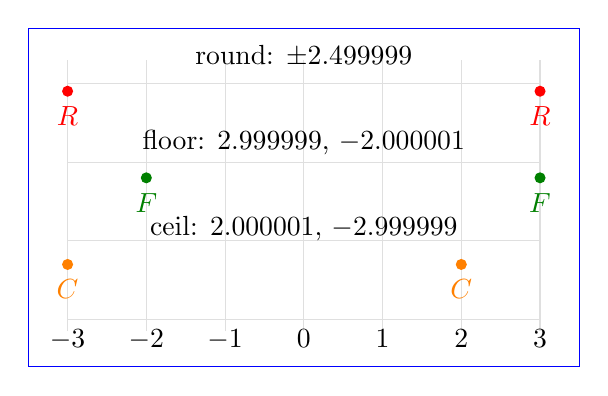
\begin{tikzpicture}
  \draw[blue] (-3.5,-.6) rectangle (3.5,3.7);
  \draw[gray!25,step=1] (-3,-.15) grid (3,3.3);
  \foreach \x in {-3,-2,-1,0,1,2,3}
    \node[below] at (\x,0) {$\x$};
  \node at (0,3.35) {round: $\pm 2.499999$};
  \node at (0,2.25) {floor: $2.999999$, $-2.000001$};
  \node at (0,1.15) {ceil: $2.000001$, $-2.999999$};
  \fill[red] ({round(2.499999)},2.9) circle (2pt) node[below=2pt] {$R$};
  \fill[red] ({round(-2.499999)},2.9) circle (2pt) node[below=2pt] {$R$};
  \fill[green!50!black] ({floor(2.999999)},1.8) circle (2pt) node[below=2pt] {$F$};
  \fill[green!50!black] ({floor(-2.000001)},1.8) circle (2pt) node[below=2pt] {$F$};
  \fill[orange] ({ceil(2.000001)},.7) circle (2pt) node[below=2pt] {$C$};
  \fill[orange] ({ceil(-2.999999)},.7) circle (2pt) node[below=2pt] {$C$};
\end{tikzpicture}
\end{document}
